\section{課題(類似画像検索システム)の概要}
\subsection{ソースコードとアルゴリズムの説明}
\begin{enumerate}
  \item 検索に使用する特徴量、キー画像の番号をキーボードから入力する。
  \begin{itemize}
    \item[→] まず、以下の図\ref{graph:1}のようにして、
    変数「検索に使用する特徴の番号」と「キー画像番号」にキーボードから入力された番号を入れる。
    \begin{figure}[htbp]
      \begin{minipage}[t]{\hsize}
        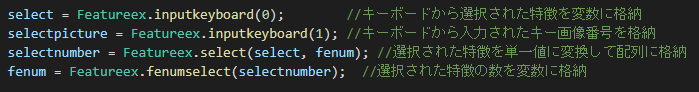
\includegraphics[scale=0.4]{キー画像入力.PNG}
        \centering
        \caption{キーボードから入力された番号を変数に格納}
        \label{graph:1}
      \end{minipage}
    \end{figure}
    \item[→] キーボードから入力された検索に使用する特徴の番号、キー画像の番号を取得するメソッドは、図\ref{graph:2}のようになっている。
    \begin{figure}[htbp]
      \begin{minipage}[t]{\hsize}
        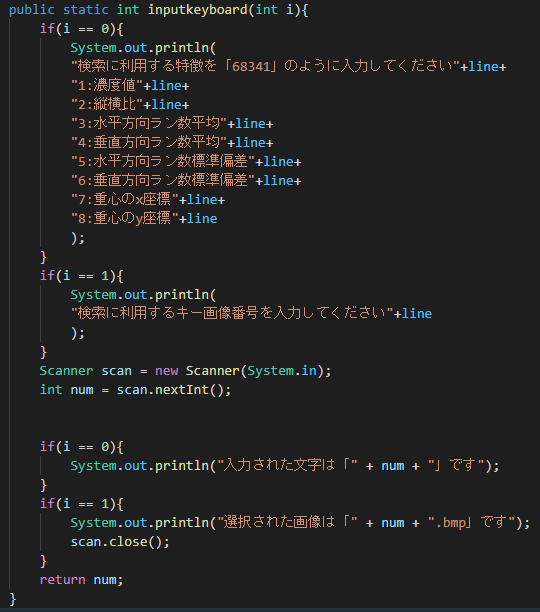
\includegraphics[scale=0.4]{キー画像入力1.PNG}
        \centering
        \caption{キーボードから入力された番号を取得するメソッド\cite{url2}}
        \label{graph:2}
      \end{minipage}
    \end{figure}
  \end{itemize}
  
  \item 100枚の画像を読み込み、特徴量を抽出する。
  \begin{itemize}
    \item[→] まず、以下の図\ref{graph:3}のようにして画像を読み込み、図\ref{graph:4}のようなメソッドを呼び出して、画像の特徴量を2次元配列に
    格納する。
    \begin{figure}[htbp]
      \begin{minipage}[t]{\hsize}
        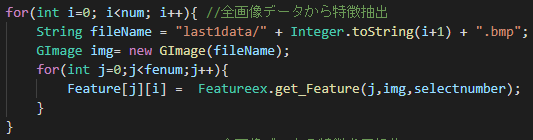
\includegraphics[scale=0.4]{画像読み込み.PNG}
        \centering
        \caption{画像を読み込み、特徴量を抽出するプログラム}
        \label{graph:3}
      \end{minipage}
    \end{figure}
    \item[→] 図\ref{graph:4}のメソッドでは、検索に使用する特徴量を判別して、対応する特徴量抽出メソッドを呼び出している。
    \begin{figure}[htbp]
      \begin{minipage}[t]{\hsize}
        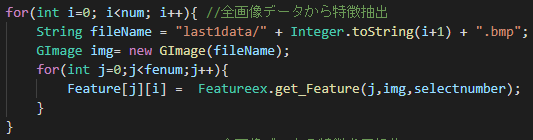
\includegraphics[scale=0.4]{画像読み込み.PNG}
        \centering
        \caption{選択された特徴の特徴量抽出メソッドを呼び出すメソッド}
        \label{graph:4}
      \end{minipage}
    \end{figure}
    \clearpage
    \item[→] 下記に各特徴量を抽出するメソッドを示す。
    \begin{itemize}
      \item 画像の濃度は以下の図\ref{graph:5}のようなメソッドで抽出する。
      \item 画像の縦横比は以下の図\ref{graph:6}のようなメソッドで抽出する。
      \item 画像の水平方向ラン数平均は以下の図\ref{graph:7}のようなメソッドで抽出する。
      \item 画像の垂直方向ラン数平均は以下の図\ref{graph:8}のようなメソッドで抽出する。
      \item 画像の水平方向ラン数標準偏差は以下の図\ref{graph:9}のようなメソッドで抽出する。
      \item 画像の垂直方向ラン数標準偏差は以下の図\ref{graph:10}のようなメソッドで抽出する。
      \item 画像の重心のx座標は以下の図\ref{graph:11}のようなメソッドで抽出する。
      \item 画像の重心のy座標は以下の図\ref{graph:12}のようなメソッドで抽出する。
      \begin{figure}[htbp]
        \begin{minipage}[t]{0.45\hsize}
          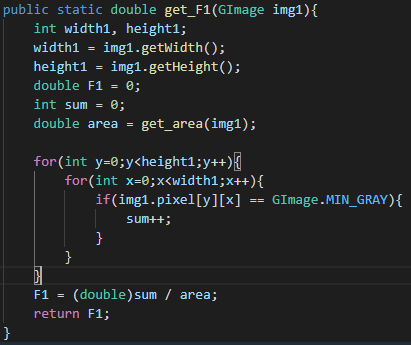
\includegraphics[scale=0.5]{濃度抽出.PNG}
          \centering
          \caption{濃度抽出メソッド}
          \label{graph:5}
        \end{minipage}
        \begin{minipage}[t]{0.45\hsize}
          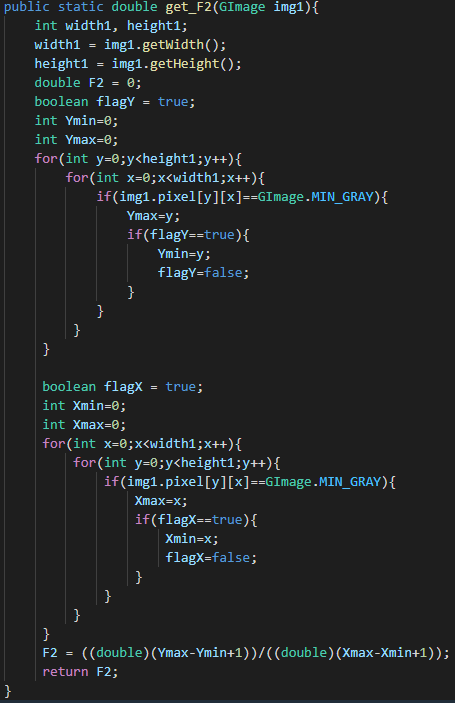
\includegraphics[scale=0.25]{縦横比抽出1.PNG}
          \centering
          \caption{縦横比抽出メソッド}
          \label{graph:6}
        \end{minipage}
        \begin{minipage}[t]{0.45\hsize}
          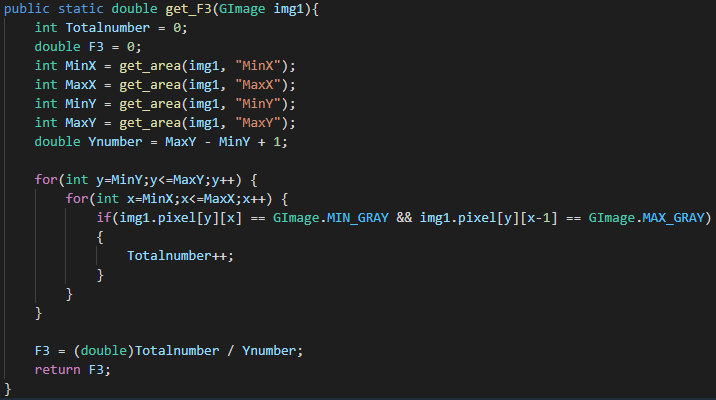
\includegraphics[scale=0.3]{水平方向ラン数平均抽出1.PNG}
          \centering
          \caption{水平方向ラン数平均抽出メソッド}
          \label{graph:7}
        \end{minipage}
        \begin{minipage}[t]{0.45\hsize}
          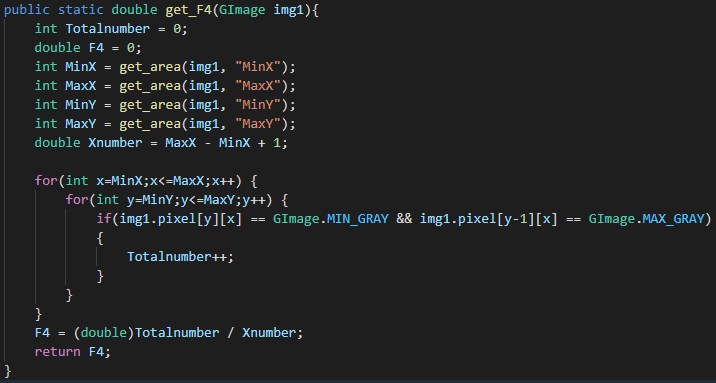
\includegraphics[scale=0.3]{垂直方向ラン数平均抽出1.PNG}
          \centering
          \caption{垂直方向ラン数平均抽出メソッド}
          \label{graph:8}
        \end{minipage}
        \begin{minipage}[t]{0.45\hsize}
          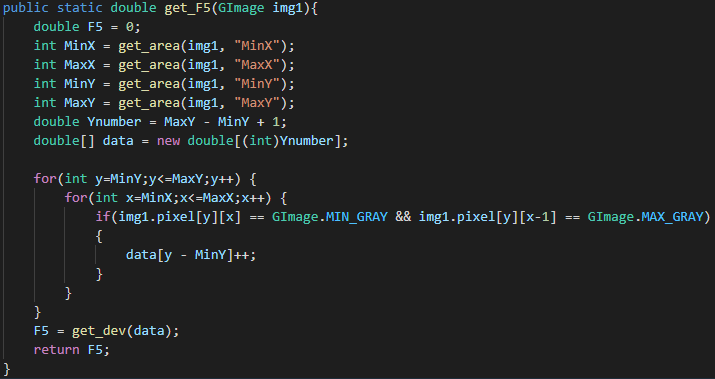
\includegraphics[scale=0.3]{水平方向ラン数標準偏差抽出1.PNG}
          \centering
          \caption{水平方向ラン数標準偏差抽出メソッド}
          \label{graph:9}
        \end{minipage}
        \begin{minipage}[t]{0.45\hsize}
          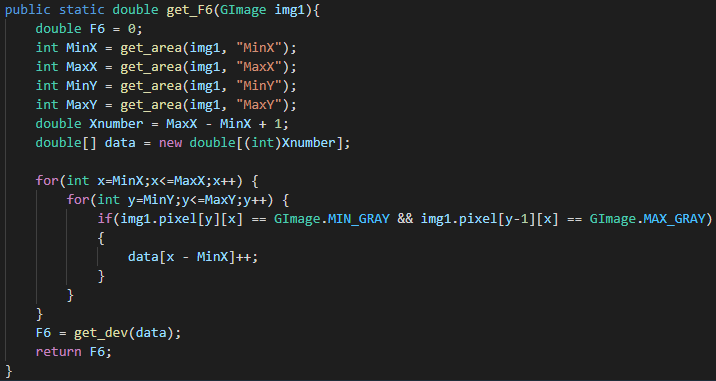
\includegraphics[scale=0.3]{垂直方向ラン数標準偏差抽出1.PNG}
          \centering
          \caption{垂直方向ラン数標準偏差抽出メソッド}
          \label{graph:10}
        \end{minipage}
        \begin{minipage}[t]{0.45\hsize}
          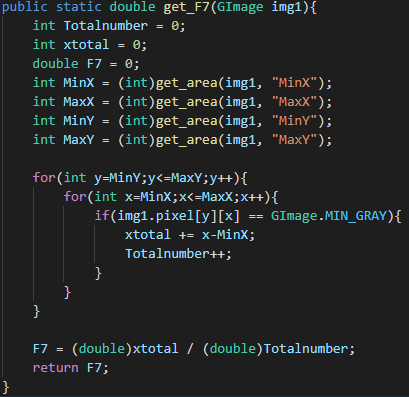
\includegraphics[scale=0.4]{重心のx座標抽出1.PNG}
          \centering
          \caption{重心のx座標抽出メソッド}
          \label{graph:11}
        \end{minipage}
        \begin{minipage}[t]{0.45\hsize}
          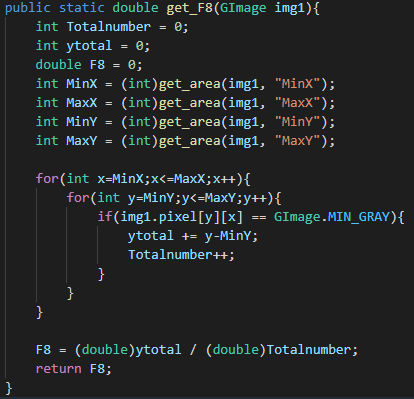
\includegraphics[scale=0.4]{重心のy座標抽出1.PNG}
          \centering
          \caption{重心のy座標抽出メソッド}
          \label{graph:12}
        \end{minipage}
      \end{figure}
    \end{itemize}
  \end{itemize}
  \clearpage

  \item 抽出した画像の特徴量を正規化する。
  \begin{itemize}
    \item[→] まず、以下の図\ref{graph:13}のようにして、
    100枚の画像の全特徴を正規化できるまで、図\ref{graph:14}のような正規化メソッドを呼び出す。
    正規化した特徴は2次元配列に格納している。
    \begin{figure}[htbp]
      \begin{minipage}[t]{0.45\hsize}
        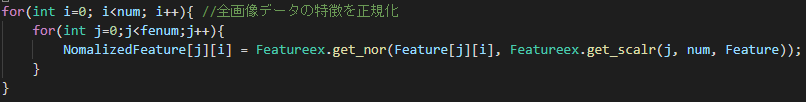
\includegraphics[scale=0.4]{画像の特徴量を正規化する.PNG}
        \centering
        \caption{全画像の全特徴を正規化するプログラム}
        \label{graph:13}
      \end{minipage}
      \begin{minipage}[t]{0.45\hsize}
        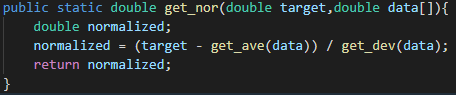
\includegraphics[scale=0.4]{画像の特徴量を正規化する1.PNG}
        \centering
        \caption{画像の特徴量を正規化するメソッド}
        \label{graph:14}
      \end{minipage}
    \end{figure}
  \end{itemize}

  \item キー画像を読み込み画像を抽出する。
  \begin{itemize}
    \item[→] 以下の図\ref{graph:15}のようにして、
    キー画像を読み込み、全画像の時と同じように特徴量を抽出して2次元配列に格納する。
    同じように、特徴量を正規化したものを2次元配列に格納する。
    \begin{figure}[htbp]
      \begin{minipage}[t]{\hsize}
        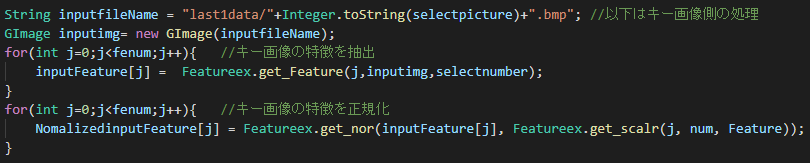
\includegraphics[scale=0.4]{キー画像読み込み.PNG}
        \centering
        \caption{キー画像を読み込み、正規化するプログラム}
        \label{graph:15}
      \end{minipage}
    \end{figure}
  \end{itemize}

  \item キー画像と全画像の距離を取得する。
  \begin{itemize}
    \item[→] まず、以下の図\ref{graph:16}のようにして、
    キー画像と全画像の距離を取得する、図\ref{graph:17}のようなメソッドを呼び出す。
    求めた距離は配列に格納している。
    \begin{figure}[htbp]
      \begin{minipage}[t]{0.45\hsize}
        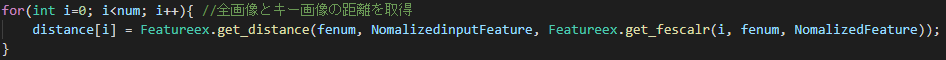
\includegraphics[scale=0.3]{キー画像と全画像の距離を取得する.PNG}
        \centering
        \caption{キー画像と全画像の距離を取得するプログラム}
        \label{graph:16}
      \end{minipage}
      \begin{minipage}[t]{0.45\hsize}
        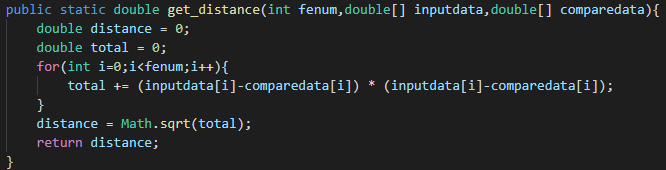
\includegraphics[scale=0.4]{キー画像と全画像の距離を取得する1.PNG}
        \centering
        \caption{キー画像と全画像の距離を取得するメソッド}
        \label{graph:17}
      \end{minipage}
    \end{figure}
  \end{itemize}
  
  \item 全画像とキー画像の距離が近い順にソートする。
  \begin{itemize}
    \item[→] まず、以下の図\ref{graph:18}のようにして、
    キー画像と全画像の距離が近い順にソートする図\ref{graph:19}のようなメソッドを呼び出す。
    また、ソートした結果の上位10個の画像番号を変数に格納する。
    \begin{figure}[htbp]
      \begin{minipage}[t]{0.45\hsize}
        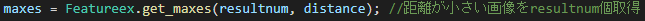
\includegraphics[scale=0.5]{昇順.PNG}
        \centering
        \caption{キー画像と全画像の距離が近い順にソートするプログラム}
        \label{graph:18}
      \end{minipage}
      \begin{minipage}[t]{0.45\hsize}
        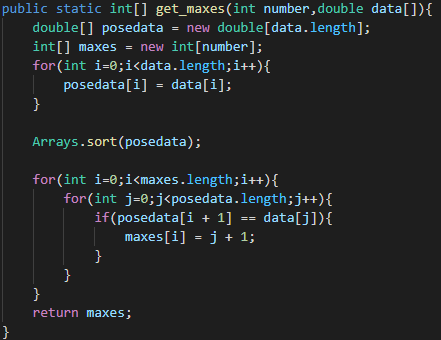
\includegraphics[scale=0.5]{昇順2.PNG}
        \centering
        \caption{キー画像と全画像の距離が近い順にソートするメソッド}
        \label{graph:19}
      \end{minipage}
    \end{figure}
  \end{itemize}
\clearpage
  \item 検索結果の画像を全てディレクトリに保存する。テキストファイルに検索結果の
  1位から10位までを出力する。また、それらの画像の検索に用いた特徴量
  、検索キーの画像番号を表示させ、その下に検索順位の上位順に結果を出す。検索結果は、検索
  順位、図形番号、(正規化前の)特徴量の値、検索キーとの距離として、10位までの画像すべて
  に対して出力する。

  \begin{itemize}
    \item[→] まず、以下の図\ref{graph:20}のようにして、
    検索結果の画像を全てディレクトリに保存する図\ref{graph:21}のようなメソッドを呼び出す。
    また、検索結果の全画像の全特徴を抽出する。
    その後、テキストファイルにテキストファイルに検索結果の
    1位から10位、それらの画像の検索に用いた特徴量
    、検索キーの画像番号を表示させ、その下に検索順位の上位順に結果、検索
    順位、図形番号、(正規化前の)特徴量の値、検索キーとの距離として、10位までの画像すべて
    に対して出力する、図\ref{graph:22}のようなメソッドを呼び出す。
    \begin{figure}[htbp]
      \begin{minipage}[t]{0.45\hsize}
        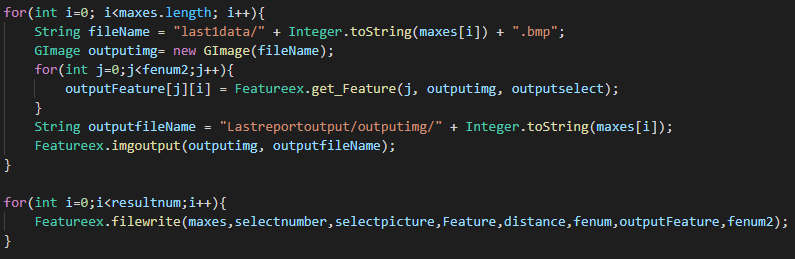
\includegraphics[scale=0.4]{ファイルに出力.PNG}
        \centering
        \caption{出力用プログラム}
        \label{graph:20}
      \end{minipage}
      \begin{minipage}[t]{0.45\hsize}
        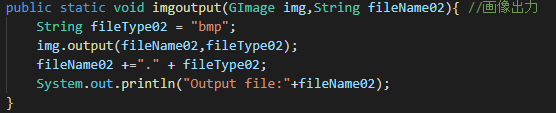
\includegraphics[scale=0.5]{画像保存.PNG}
        \centering
        \caption{画像をディレクトリに保存するメソッド}
        \label{graph:21}
      \end{minipage}
      \begin{minipage}[t]{\hsize}
        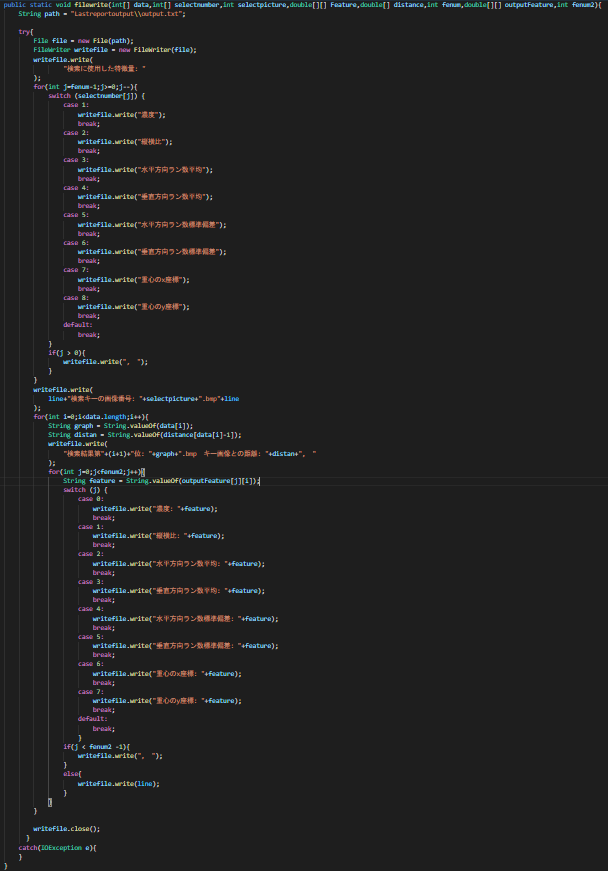
\includegraphics[scale=0.6]{テキストファイルに書き込む.PNG}
        \centering
        \caption{テキストファイルに書き込むメソッド\cite{url1}}
        \label{graph:22}
      \end{minipage}
    \end{figure}
  \end{itemize}
\end{enumerate}
\clearpage
その他、課題で使用したメソッド
\begin{itemize}
  \item 以下の図\ref{graph:23}のメソッドは、配列の平均を返す。
  \item 以下の図\ref{graph:24}のメソッドは、配列の標準偏差を返す。
  \item 以下の図\ref{graph:25}のメソッドは、画像の外接矩形の端の四辺を返す。
  \item 以下の図\ref{graph:26}のメソッドは、画像の外接矩形の面積を返す。
  \item 以下の図\ref{graph:27}のメソッドは、2次元配列を1次元配列に変換する。
  \item 以下の図\ref{graph:28}のメソッドは、キーボードから入力された特徴の番号を配列化したものと選ばれた特徴の数を返す。
  \begin{figure}[htbp]
    \begin{minipage}[t]{0.45\hsize}
      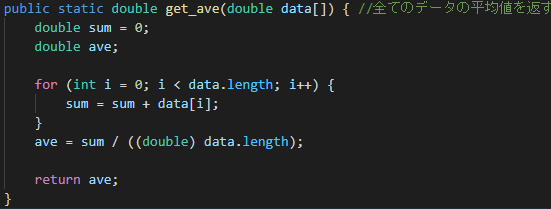
\includegraphics[scale=0.5]{平均.PNG}
      \centering
      \caption{平均を返すメソッド}
      \label{graph:23}
    \end{minipage}
    \begin{minipage}[t]{0.45\hsize}
      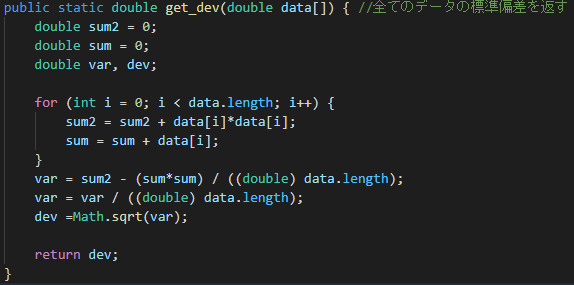
\includegraphics[scale=0.5]{その他2.PNG}
      \centering
      \caption{標準偏差を返すメソッド}
      \label{graph:24}
    \end{minipage}
    \begin{minipage}[t]{0.45\hsize}
      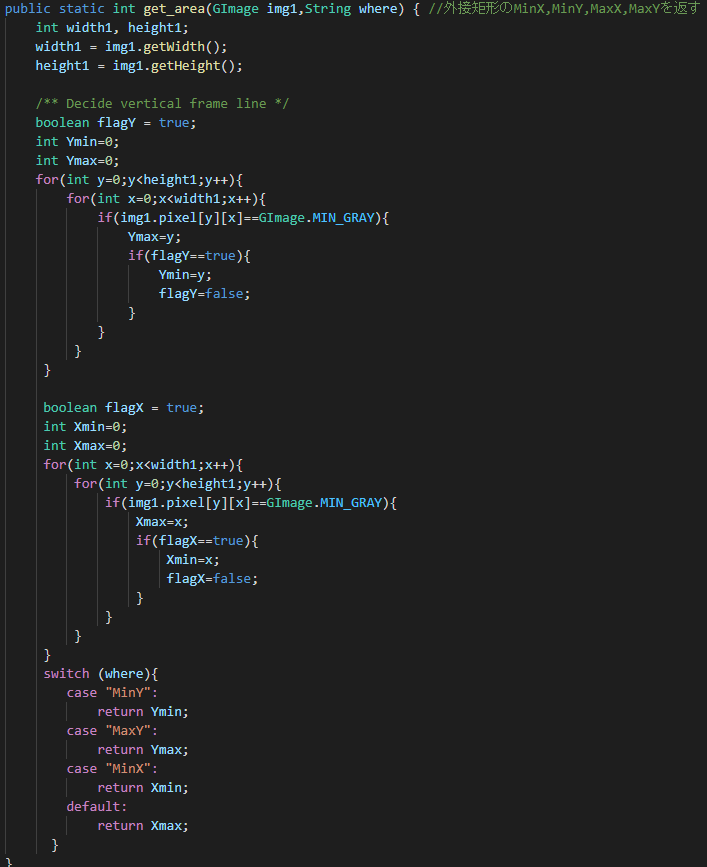
\includegraphics[scale=0.3]{その他3.PNG}
      \centering
      \caption{外接矩形の端の四辺を返すメソッド}
      \label{graph:25}
    \end{minipage}
    \begin{minipage}[t]{0.45\hsize}
      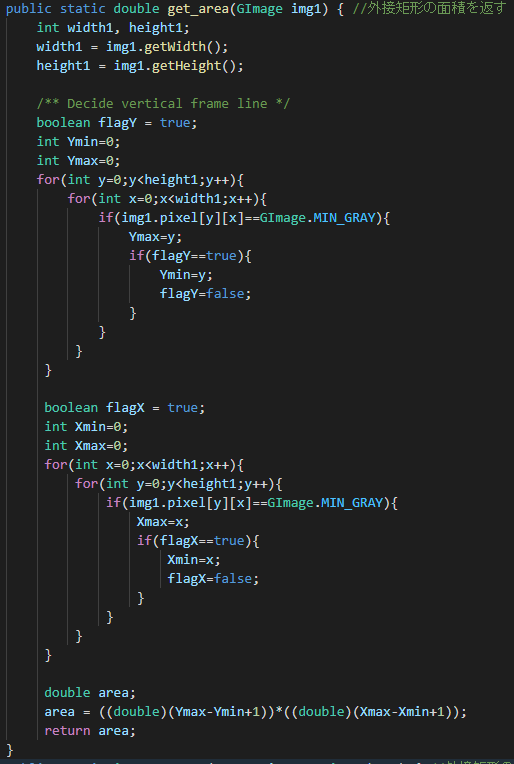
\includegraphics[scale=0.3]{その他4.PNG}
      \centering
      \caption{外接矩形の面積を返すメソッド}
      \label{graph:26}
    \end{minipage}
    \begin{minipage}[t]{0.45\hsize}
      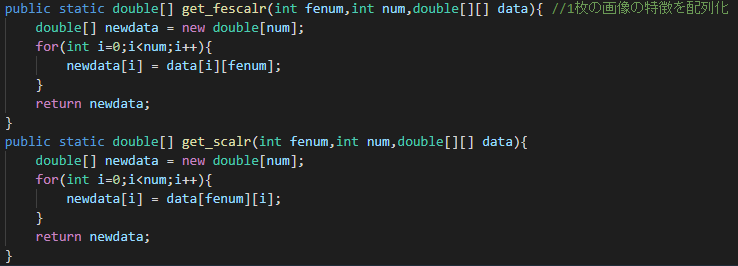
\includegraphics[scale=0.4]{その他5.PNG}
      \centering
      \caption{2次元配列を1次元配列に変換するメソッド}
      \label{graph:27}
    \end{minipage}
    \begin{minipage}[t]{0.45\hsize}
      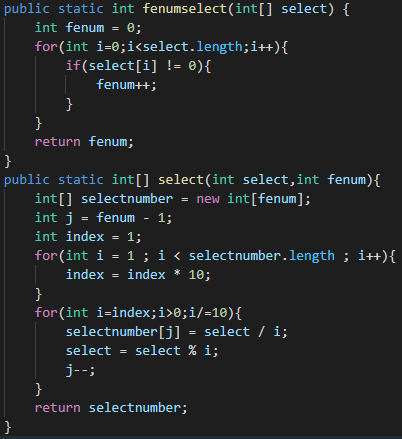
\includegraphics[scale=0.5]{その他6.PNG}
      \centering
      \caption{特徴の番号を配列化したものと選ばれた特徴の数を返すメソッド}
      \label{graph:28}
    \end{minipage}
  \end{figure}
\end{itemize}
\clearpage

\subsection{何を入力して、どのように出力されるのか}
\begin{enumerate}
  \item プログラムを実行するとコンソールに図\ref{graph:29}のような画面が表示される。
  \item 指示通りに検索に使う特徴量の番号を入力すると図\ref{graph:30}のような画面が表示される。
  \item 次に、キー画像番号を入力すると図\ref{graph:31}のような画面が表示される。
  \item コンソールに表示されたディレクトリを開くと図\ref{graph:32}のようになっている。
  \item ディレクトリにあるテキストファイル「output.txt」を開くと図\ref{graph:33}のようになっている。
  内容は、画像の検索に用いた特徴量、検索キーの画像番号、
  その下に検索順位の上位順に結果があり、その横には検索
  順位、図形番号、(正規化前の)特徴量の値、検索キーとの距離がある。
  \item もう一つのディレクトリ「outputimg」を開くと図\ref{graph:34}のようになっており、
  中にある画像は、すべて検索結果の画像となっている。
  \begin{figure}[htbp]
    \begin{minipage}[t]{0.33\hsize}
      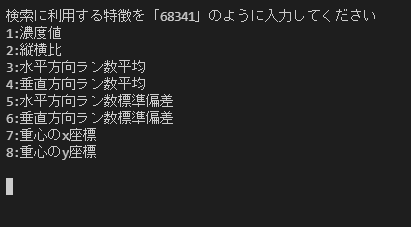
\includegraphics[scale=0.4]{入力1.PNG}
      \centering
      \caption{コンソールの初期画面}
      \label{graph:29}
    \end{minipage}
    \begin{minipage}[t]{0.33\hsize}
      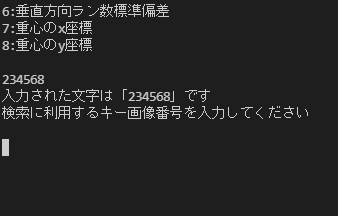
\includegraphics[scale=0.4]{入力2.PNG}
      \centering
      \caption{検索に使用する特徴入力後}
      \label{graph:30}
    \end{minipage}
    \begin{minipage}[t]{0.33\hsize}
      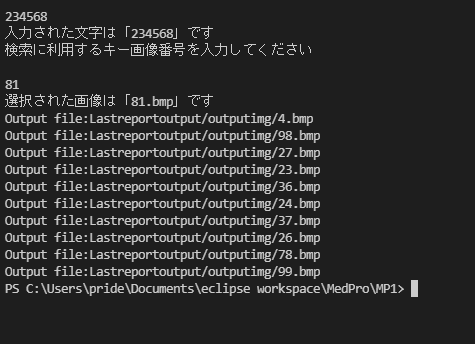
\includegraphics[scale=0.4]{入力3.PNG}
      \centering
      \caption{キー画像番号入力後}
      \label{graph:31}
    \end{minipage}
    \begin{minipage}[t]{0.33\hsize}
      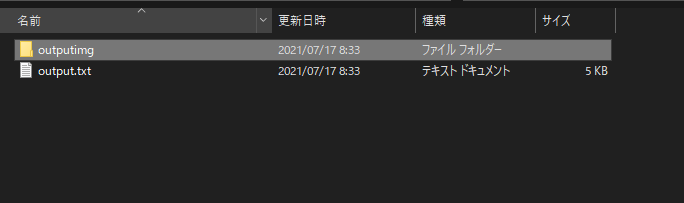
\includegraphics[scale=0.35]{入力4.PNG}
      \centering
      \caption{出力ディレクトリの中身}
      \label{graph:32}
    \end{minipage}
    \begin{minipage}[t]{0.66\hsize}
      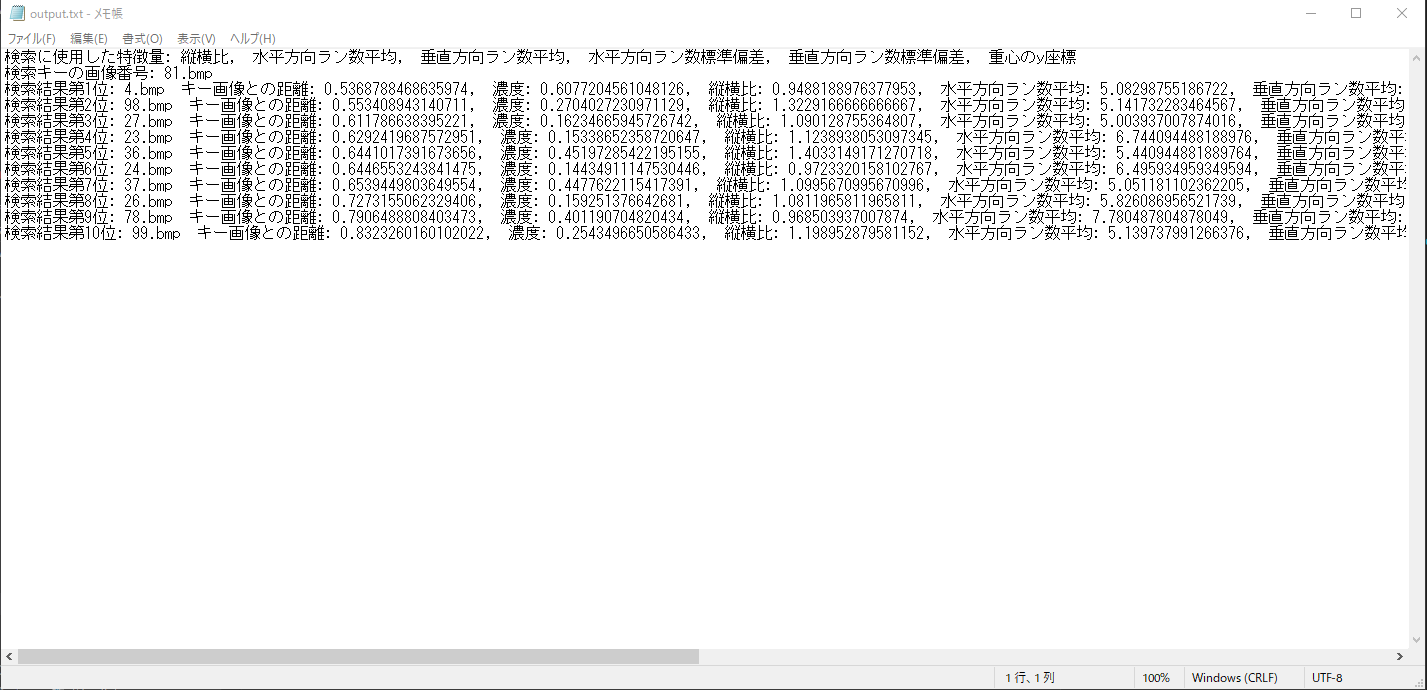
\includegraphics[scale=0.25]{入力5.PNG}
      \centering
      \caption{output.txtの中身}
      \label{graph:33}
    \end{minipage}
    \begin{minipage}[t]{\hsize}
      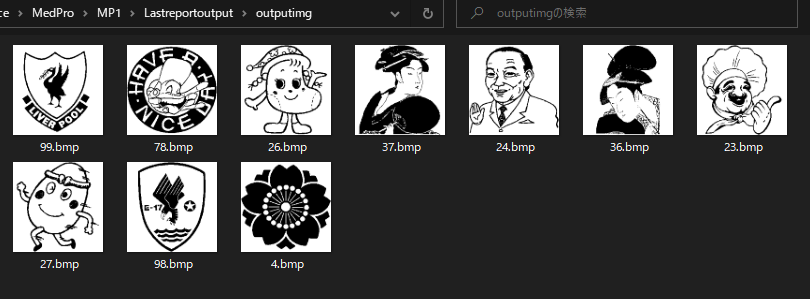
\includegraphics[scale=0.6]{入力6.PNG}
      \centering
      \caption{outputimgの中身}
      \label{graph:34}
    \end{minipage}
  \end{figure}
\end{enumerate}
